%
% Transportation Research Board conference paper template
% version 3.1 Lite
%
% When numbered option is activated, lines are numbered.
\documentclass[numbered]{trbunofficial}
\usepackage{graphicx}
\usepackage[ruled, linesnumbered]{algorithm2e}
\DecMargin{0.65cm}
\SetAlCapHSkip{5pt}
\usepackage{morefloats}
\usepackage{color}
\usepackage{amsfonts}
\usepackage{amsmath}
\usepackage{breqn}
\usepackage{array}
\usepackage{tabularx}
\usepackage{siunitx}
\sisetup{tight-spacing=true, free-standing-units=true, use-xspace=true, space-before-unit=true}
\newcommand{\sidiv}{/\hspace{-1.5pt}} % if unit like m/s add divide and pull back space after second unit
%\usepackage{nomencl}
%\makenomenclature
\usepackage{rotating}
\usepackage{threeparttable, multirow}
\usepackage{hhline}% http://ctan.org/pkg/hhline
\usepackage{verbatim}
%\usepackage[bookmarks=false]{hyperref}
\usepackage{scrextend}
%\usepackage{lscape}
%\usepackage[square,sort,comma,numbers]{natbib}
\usepackage[font=small]{caption}
\usepackage{listings}
\usepackage{booktabs}
\usepackage{afterpage}
\newcommand{\tabitem}{~~\llap{\textbullet}~~}
\usepackage{pdflscape}


% \usepackage[colorlinks=true,linkcolor=blue,citecolor=blue]{hyperref}
% For TRB version hide links
%\usepackage[hidelinks]{hyperref}
\usepackage{nohyperref}

\makeatletter
\g@addto@macro\normalsize{%
	\setlength\abovedisplayskip{10pt}
	\setlength\belowdisplayskip{10pt}
	\setlength\abovedisplayshortskip{10pt}
	\setlength\belowdisplayshortskip{10pt}
}
\makeatother

%ltable
\newenvironment{ltable}
{\begin{landscape}\begin{table}}
		{\end{table}\end{landscape}}

% Put here what will go to headers as author
\AuthorHeaders{Rafter and Anvari}
\title{Hybrid Traffic Responsive Control for\newline Isolated Signalised Intersections}

% TODO: add macros for easier formatting of \author.
\author{%
  \textbf{Craig B. Rafter*}\\
	Transportation Research Group\\
	University of Southampton\\
	Faculty of Engineering and the Environment\\
	Southampton, SO16 7QF, United Kingdom\\
	Email: c.b.rafter@soton.ac.uk\\
  \hfill\break% this is a way to add line numbering on empty line
  \hfill\break%
  \textbf{Bani Anvari, Ph.D.}\\
	Transportation Research Group\\
	University of Southampton\\
	Faculty of Engineering and the Environment\\
	Southampton, SO16 7QF, United Kingdom\\
	Email: b.anvari@soton.ac.uk\\
	\hfill\break\hfill\break
	\textbf{Simon Box, Ph.D.}\\
	Transportation Research Group\\
	University of Southampton\\
	Faculty of Engineering and the Environment\\
	Southampton, SO16 7QF, United Kingdom\\
	Email: s.box@soton.ac.uk\\
	\hfill\break\hfill\break
	\textbf{*} \emph{Corresponding author}
}

% If necessary modify the number of words per table or figure default is set to
% 250 words per table and figure
% \WordsPerTable{250}
% \WordsPerFigure{250}

% If words are counted manually, put that number here. This does not include
% figures and tables. This can also be used to avoid problems with texcount
% program i.e. if one does not have it installed.
% \TotalWords{200}

\begin{document}
\begin{nolinenumbers}
	\maketitle
\end{nolinenumbers}


\section{Abstract}

This paper compares the performance a traffic responsive hybrid signalised intersection controller which combines vehicle GPS and inductive loop information, to fixed-time, inductive loop, and GPS based controllers. 
Road users spend up to 42\% of their time in congested traffic. 
Inefficient signal timing choices by intersection controllers contribute to traffic delays, causing severe negative impacts on the economy and environment. 
Signal timings can be improved using vehicles' GPS information combined with vehicle flow information from inductive loops to overcome the control action deficit at isolated intersections. 
This new signal control algorithm is beneficial for traffic engineers and governmental agencies, as traffic flow can be optimised, therefore, reducing fuel consumption and emissions.

Under the open European Telecommunication Standards Institute (ETSI) Cooperative Awareness Message (CAM) framework, a traffic responsive Hybrid Vehicle Actuation algorithm (HVA) is proposed. HVA uses position and heading data from vehicle status broadcasts, and inferred velocity information to determine vehicle queue lengths and detect vehicles passing through the intersection. When vehicle broadcast data are unavailable, inductive loop data are used. The gathered information is used to actuate intersection signal timings.
Microscopic simulations comparing HVA to fixed-time control, inductive loop based vehicle actuation (Loop-VA) and GPS based vehicle actuation (GPS-VA) on four urban road networks were performed to see how the proposed HVA algorithm performs compared to existing control strategies. 
The results show that HVA is an effective alternative to traditional intersection control strategies, offering delay reductions of up to ${50\%}$ over Loop-VA.

\hfill\break%
\noindent\textit{Keywords}: Intelligent Transport Systems, Traffic Control, Connected Vehicles
\newpage

\section{Introduction}\label{sec:intro}
% Motivation
Traffic delays are a significant problem in developed vehicle markets. In the UK, Germany, and US alone, traffic congestion cost their economies a combined \$450 billion in lost time and wasted energy~\cite{inrixgts17}.
% Previous Work
Traffic congestion can be mitigated through responsive control of signalised intersections. From simple control schemes such as fixed-time (e.g. TRANSYT~\cite{robertson69}) or vehicle actuation, to more sophisticated adaptive control schemes such as SCOOT~\cite{hunt1981} and MOVA~\cite{vincent88}, signalised intersection control is important for managing the network demand~\cite{papageorgiou2003}. 

Intelligent Transport Systems (ITS) are the integration and application of communication systems, data driven control strategies, and large-scale information processing to transport systems. Many of the hypothesised traffic control schemes for ITS assume ideal communication between vehicles and infrastructure, or require the dominant presence of autonomous or connected vehicles in the network~\cite{goodall2013, Au2015, HomChaudhuri2016}. 

Connected and Autonomous Vehicles (CAVs) are predicted to be introduced from 2020 onward and it will take time for the vehicle fleet to turnover~\cite{litman2016}. Therefore, there is a need for strategies that can modify existing infrastructure and support the transport network as it becomes increasingly automated. CAV centric control schemes will be needed eventually. However, as vehicles are incrementally modernised, it is important that traffic control strategies adapt according to the vehicle fleet composition, and fairly consider all types of road users.

This paper focuses on control strategies for connected vehicles (CVs). CVs are those which transmit and receive information from vehicles and infrastructure equipped with communication systems. Having multiple classes of vehicles has been shown to have negative effects on the resulting traffic flow~\cite{Ngoduy2012, Ngoduy2014}, and is taken into account.

% This Work
This paper contributes the HVA algorithm which uses position and heading data from vehicle status broadcasts, and inferred velocity information to actuate signal timings. The signal timings are adjusted by predicting vehicle queue lengths in stopped lanes, and detecting vehicles passing through the junction on lanes in their green cycle. When information vehicle status broadcasts is sparse, data from inductive loops are used to actuate the signal timings. The data are transferred from the vehicles to the intersections using the IEEE 802.11p communication protocol~\cite{ieee80211p}, and the ETSI Cooperative Awareness Message (CAM) framework~\cite{EtsiCAM2011} in order to ensure interoperability among connected vehicle implementations. The proposed HVA scheme is tested and compared in simulations to fixed-time control, Loop-VA, and GPS-VA on four common urban road networks (A T-junction, twin T-junction, corridor, and Manhattan grid). %The results show that GPS-VA is an effective alternative to traditional intersection control strategies, GPS-VA is a compelling alternative to traditional intersection control strategies, showing delay reductions of $10\%-50\%$ over vehicle actuation for connected vehicle penetrations exceeding $30\%$.

% Contents
This paper is organised as follows: The first section discusses the background literature regarding existing intersection control strategies. Then the fixed-time, Loop-VA, GPS-VA, and HVA intersection control algorithms are defined. Next, the simulation procedure used to compare the algorithm to existing methods is outlined, and the simulation results are presented and discussed. Finally, conclusions are drawn and avenues for further research are discussed.

\section{Background}\label{sec:bg}
An abundance of signal control strategies have been developed with the intent of improving traffic flow and reducing delays at signalised intersections. Table \ref{tab:traffctrl} outlines a selection of control strategies commonly used in urban environments under the three key classes of intersection controller. Namely isolated, coordinated fixed-time, and coordinated traffic-responsive control. For each class of controller the operation of the control strategy is summarised, and references to the key literature for the strategy are given. Table \ref{tab:traffctrl} builds upon the review of traffic control strategies by \cite{papageorgiou2003}, and is followed by a review of ITS control strategies. The common distinctions of signal control strategies are:
\begin{itemize}
	\item The strategy controls an intersection, or network of intersections.
	\item An intersection comprises several approaches, each of which contain one or more lanes.
	\item Each lane has an associated queue and vehicle flow.
	\item Measurement of the vehicle flow typically occurs locally via inductive loops, or video systems.
	\item A phase is an indication of movement priority on a particular lane (i.e. green to go, or red to stop for example).
	\item A stage defines a set of non-conflicting phases.
\end{itemize}
Additionally, there are four key terms needed to understand intersection control:
\begin{itemize}
	\item \emph{Isolated control} - The intersections in the network are controlled independently. This can be useful for small or sparsely distributed networks. 
	\item \emph{Coordinated control} - Coordinated strategies control multiple junctions. The idea is to create \emph{`green waves'} so that traffic lights go green along several routes in the same direction to maximise vehicle throughput along a particular road section. 
	\item \emph{Fixed-time control} - Fixed-time strategies use pre-determined stages and timings that can be equally or proportionally split between routes, or based on calculations done off-line using historical vehicle data. The timings may vary according to time of day (during rush hours for example).
	\item \emph{Traffic-responsive control} - Strategies of this class control multiple junctions, performing on-line optimisation of signal timings and stage configurations based on network demand using real-time traffic data. 
\end{itemize}

\afterpage{\begin{ltable}[p]
		\small
		\caption{Summary of key urban traffic control strategies.}
		{\begin{threeparttable}
				\begin{tabular}{p{3.1cm}p{2.9cm}p{12.5cm}p{2.0cm}}
					\toprule
					\textbf{Controller Class} & \textbf{Control Strategy} & \textbf{Strategy Information} &\textbf{References} \\
					\toprule
					\multirow{5}{4cm}{Isolated Intersection} & 
					Fixed-Time & 
					\tabitem Cycles through pre-determined stage times & \multirow{3}{4cm}{\cite{allsop1971, allsop1975, allsop1976, allsop1981}} \\&&
					\tabitem Inflexible to varying demand \\&&
					\tabitem Examples include SIGSET and SIGCAP
					\\\cmidrule{2-4}&
					\multirow{2}{2.75cm}{Traffic-Responsive} & 
					\tabitem Uses real-time inductive loop data to actuate stage times & \multirow{2}{4cm}{\cite{miller1963, vincent88, peirce1990}} \\&&
					\tabitem Most notably, Miller's strategy implemented as part of MOVA\\
					\midrule
					\multirow{8}{3cm}{Coordinated Fixed-Time} & 
					\multirow{1}{2.75cm}{MAXBAND/ MULTIBAND} & 
					\tabitem Selects signals from a set of possible signals such as to maximise the number\newline\hphantom{\tabitem}of vehicles that can pass through the intersection without stopping & \multirow{3}{4cm}{\cite{little1966, cohen1982, stamatiadis1996}} \\&&
					\tabitem Chooses the signal and stage time to maximise the system bandwidth
					\\\cmidrule{2-4}&
					\multirow{2}{2.75cm}{TRANSYT/ TRANSYT-7F} & 
					\tabitem Calculates a performance index based primarily on delays and stops & \multirow{3}{3cm}{\cite{robertson69, li1999}} \\&&
					\tabitem Optimises the signal timings to minimise the performance index based on\newline\hphantom{\tabitem}historical inductive loop data.
					\\\cmidrule{2-4}&
					PASSER IV & 
					\tabitem Aims to optimise progression band with for multi-arterial road traffic & \multirow{2}{4cm}{\cite{chaudhary1993}} \\&&
					\tabitem Optimizes cycle lengths, offsets, and phase sequencing.\\
					\midrule
					\multirow{15}{4cm}{Coordinated Traffic-Responsive} & 
					SCOOT/SCATS & 
					\tabitem Uses real-time data to optimise traffic flow between multiple intersections & \multirow{1}{4cm}{\cite{hunt1981, lowrie1990}}
					\\\cmidrule{2-4}&
					Model-Based \newline Optimisation & 
					\tabitem Uses real-time traffic data to dynamically optimise the switching values for\newline\hphantom{\tabitem}the next few stage times & \multirow{3}{4cm}{\cite{gartner1983, henry1984, boillot2006, mirchandani2001}} \\&&
					\tabitem Examples include OPAC, PRODYN, CRONOS, RHODES
					\\\cmidrule{2-4}&
					Store-and-Forward & 
					\tabitem Describes traffic flow without discrete variables allowing for more\newline\hphantom{\tabitem}efficient optimisation routines to be used & \multirow{3}{4cm}{\cite{diakaki1999,diakaki2002,gazis2006,gazis1963}} \\&&
					\tabitem Implemented in the TUC traffic controller
					\\\cmidrule{2-4}&
					REALBAND & 
					\tabitem Identifies and predicts the movement of vehicle platoons through the\newline\hphantom{\tabitem}transport network & \multirow{4}{4cm}{\cite{dellolmo1995}} \\&&
					\tabitem Signals times are allocated to the predicted platoons based on the\newline\hphantom{\tabitem}optimisation of a performance criterion
					\\\cmidrule{2-4}&
					ALLONS-D & 
					\tabitem Real-time decentralised traffic-responsive delay minimiser with implicit\newline\hphantom{\tabitem}coordination & \multirow{4}{4cm}{\cite{porche1997}} \\&&
					\tabitem Can generate non-cyclic paths. Allows arbitrary phase sequencing/splits\newline\hphantom{\tabitem}within the constraints of a minimum and maximum green time.
					\\\bottomrule
				\end{tabular}
				\begin{tablenotes}[flushleft]
					\item \emph{}
				\end{tablenotes}
			\end{threeparttable}}\label{tab:traffctrl}
		\end{ltable}}
		
\afterpage{\begin{ltable}[p]
\small
\caption{Summary of key ITS traffic control strategies.}
{\begin{threeparttable}
		\begin{tabular}{p{2.cm}p{0.01cm}@{}p{20cm}}
			\toprule
			\multirow{2}{2.0cm}{\textbf{Key Literature}} & \textbf{} & \multirow{2}{10cm}{\textbf{Control Strategy Information}} \\\\
			\toprule
			\multirow{1}{3.5cm}{\cite{goodall2013, smith2010}} &	& 
			\tabitem Traffic-responsive decentralized isolated intersection control strategy \\&&
			\tabitem Determines vehicle queue length using GPS data from vehicles \\&&
			\tabitem Sets green time based on the time to clear the queue or for the queue to reach a target speed \\
			\midrule
			
			\multirow{1}{4.5cm}{\cite{Fajardo2011, Au2015}} &	& 
			\tabitem Traffic-responsive isolated centralized strategy\\&&
			\tabitem Vehicles make reservations with a central server that directs them through the intersection \\&&
			\tabitem Vehicles are directed on a first-come-first-served basis \\&&
			\tabitem Does not require traffic lights in a fully autonomous system, traffic lights are only used to direct human drivers \\
			\midrule
			
			\cite{HomChaudhuri2016} &	&
			\tabitem Uses V2V communication to relay signal phase and timing (SPaT) information to vehicles \\&&
			\tabitem Connected vehicles with sufficient automation adjusts their velocity so as to still be in motion when the  traffic light turns green \\
			\midrule
			
			\cite{He2012, He2014} & & 
			\tabitem The authors present Platoon-based Arterial Multi-modal Signal Control with Online Data (PAMSCOD) \\&&
			\tabitem An intersection manager receives travel mode, position, speed, and desired phase information from the vehicle \\&&
			\tabitem The requests are then optimised to determine the next phase and timings\\
			\midrule
			
			\cite{priemer2009} &	& 
			\tabitem Uses vehicle speed and position data to optimise the phase every 5 seconds \\&&
			\tabitem The optimisation procedure attempts to reduce the queue length over 20 forecasted seconds \\&&
			\tabitem Provisions priority access strategies for special vehicles or traffic streams \\
			\midrule
			
			\cite{Datesh2011} &	& 
			\tabitem The authors present the IntelliGreen Algorithm \\&&
			\tabitem Uses k-means clustering to determine when the phase should change (k=2, enumerated red/green) \\&&
			\tabitem Vehicles are grouped into clusters based on their time-to-intersection (based on received speed, position data) \\&&
			\tabitem Green time is set based on the largest time-to-intersection of all the vehicles in the green cluster\\
			\midrule
			
			\cite{Lee2013} &	& 
			\tabitem A traffic responsive method that uses cumulative travel time (CTT) data from connected vehicles \\&&
			\tabitem CTT accumulated from when vehicles begin their approach to the intersection \\&&
			\tabitem Sets the signal phase and green time based on the phase with the highest total CTT \\
			\midrule
			
			\cite{Lee2012} &	& 
			\tabitem A connected vehicle intersection coordination scheme is proposed that requires 100\% connected vehicles \\&&
			\tabitem Vehicles may proceed through the intersection without stopping by determining safe gaps between itself and the other vehicles \\
			\midrule
			
			\cite{yang2016} &	& 
			\tabitem Proposes an algorithm requiring minimal driver assistance that results in self-organised, decentralised traffic flow. \\&&
			\tabitem Vehicles synchronise their approaches so as to pass through the intersection without collision \\
			\bottomrule
		\end{tabular}
		\begin{tablenotes}[flushleft]
			\item \emph{}
		\end{tablenotes}
	\end{threeparttable}}\label{tab:itsctrl}
\end{ltable}}
				
Intersection control is a widely studied area, the current developments in the area of autonomous vehicle and ITS technologies offer a renewed opportunity to improve on the prevalent control strategies discussed previously, and even develop new strategies that harness ITS data streams.

Table \ref{tab:itsctrl} compiles notable ITS intersection control strategies, some of which are discussed in detail in \cite{feng2015}. Table \ref{tab:itsctrl} provides references to the authors of the control strategy, and the key points about how the proposed control strategy differs from existing strategies, and harnesses the ITS data stream. It can be seen that communication is a key feature of all of the strategies and that shared information facilitates the development of strategies that do not rely solely on loop data.

There is a significant gap between the prevalent traffic control strategies and the ITS control strategies. The prevalent strategies do not harness the ITS data stream at all, and it needs to be investigated whether this information is beneficial for traffic control. Furthermore, the ITS based strategies typically rely on idealised communications and high penetrations of CAVs. The reliance on communication systems leaves them ill-prepared to deal with mixed human driver-CAV fleets, and their robustness to communication errors unknown. 

\section{Intersection Control Strategies}\label{sec:ctrllog}
In this section, the developed intersection control schemes are described. First, some terminology is introduced and the algorithms for the fixed-time and vehicle actuation benchmark intersection controllers are presented. An algorithm which uses GPS data to perform vehicle actuation is then proposed. Finally, an algorithm that incorporates elements from both the loop based and GPS based control is developed.

% The fundamental difference between unconnected and connected vehicles (CVs) is in how they interact with infrastructure. Unconnected vehicles rely solely on the driver's immediate interpretation of their environment. In contrast, an ITS communicates additional information to and from its environment, and is able to inform not only its reaction to the current situation, but also its future decisions. The challenge is in determining whether the system should use a top-down approach, where the intersection is managed by a master controller, or a bottom-up approach, where the traffic dynamics are governed locally by each vehicle contributing to create a net effect. A combination of the two can be achieved, but the scope of the designed methods will be fundamentally limited by the standards imposed on the system.

Traffic stages are defined as the traffic lights configuration at an intersection. Table~\ref{tab:tlType} defines the possible phases a traffic light can have and their meanings. Here, a stage comprises the set of traffic phases that give priority green to a single side of intersection. The side of the junction showing priority green will be referred to as the `active side', the others are considered `inactive'. Inactive lanes display permissive green on routes that are not in conflict any priority green streams, and red on streams that conflict with priority stream(s). Pedestrians are not considered so stages only account for vehicle presence.

\begin{table}[htb]
	\small
	\centering
	\caption{Traffic light phase definitions.\vspace{-1.0ex}}
	\begin{tabular}{p{2.5cm}p{7cm} }
		\toprule
		\textbf{Phase} & \textbf{Description} \\ \toprule
		Red & Vehicles must stop \\ \midrule
		Yellow & Vehicles stop if it is safe to do so \\ \midrule
		\multirow{2}{2.5cm}{Permissive Green} & Vehicles proceed if the road is unoccupied by vehicles in a priority green stream \\ \midrule
		Priority Green & Vehicles proceed if it is safe to do so \\ 
		\bottomrule
	\end{tabular}
	\label{tab:tlType}
\end{table}

All of the algorithms presented in this paper make control decisions every $h$ seconds, where $h=1\second$ for all strategies.  Where CVs send data, the data are sent at a rate of $10\Hz$ per the ETSI CAM~\cite{EtsiCAM2011}  specification. Messages are sent over an IEEE 802.11p~\cite{ieee80211p} Dedicated Short-Range Communication (DSRC) Research on IEEE 802.11p networks shows that signal strength within a $250\m$ range is high enough that messages can be received correctly~\cite{msadaa2010, hameedmir2014}, and that packet latencies of approximately $50\ms$ are achievable at vehicles speeds up to $90\km\sidiv\hour$~\cite{msadaa2010}. In this paper CAMs are received by the intersection controller with ideal information content, but with a delay of $100\ms$. The fixed-time, Loop-VA and GPS-VA were the subject of an earlier study by \trbcite{rafter2017}, the difference being control was done at the resolution of $h=0.1\second$ the same as the simulation time step

\subsection{Existing Algorithms}
\subsubsection{Fixed-time Control}
Fixed-time control is the most basic form of automated signal control. Each side of the intersection is set active for a predetermined amount of time, and the controller cycles through the stages sequentially. Algorithm~\ref{alg:ft} is the pseudocode description of the fixed-time control process. Fixed-time control is relatively simple to implement but is not inherently adaptive or responsive, and cannot be optimised beyond calibrating the timings using historic traffic flow data.

%The phases only define the green/red states, if a traffic light transitions from red to green or vice-versa, the light turns yellow for three seconds~\cite{theSTM2008} as an intermediates step to the transition. %The stage times usedfor fixed-time control implementation are static.

\begin{algorithm}[h]
	\caption{Fixed-Time Control Algorithm Pseudocode}
	\label{alg:ft}
	\SetAlgoVlined
	\SetVlineSkip{3pt}
	%\SetAlgoNoEnd
	\Begin(Fixed-time control){
		\eIf{elapsedTime $<$ stageDuration}{
			elapsedTime $\gets$ elapsedTime$\,+\,$timeStep
		}
		{ 
			\textbf{DO:} change to next traffic stage\\
			elapsedTime $\gets$ 0
		}
	}
\end{algorithm}
\setlength{\textfloatsep}{2pt}

\subsubsection{Loop Based Vehicle Actuation} \label{sec:va}
Loop-VA uses inductive loops \cite{Yauch1990} to detect traffic and responsively adjust stage durations according to the traffic demand detected at the intersection.

In this paper, a fully-actuated intersection control strategy is implemented under Federal Highways Administration Signal Timing Manual (STM)~\cite{theSTM2008} guidelines for Loop-VA. Loop-VA systems can skip stages if they do not detect vehicles in the lane(s) corresponding to those stages; however, in order to make the Loop-VA scheme comparable to the GPS-VA scheme presented in Section~\ref{sec:gpsva}, a minimum green time is defined. 
The STM specifies that the minimum green time of between $7$ and $16\s$ for major arterial roads, and between $4$ and $10\s$ for minor arterial roads satisfies driver expectancy and queue clearance criteria for speed limits up to $50\km\sidiv\hour$. As the models used contain both minor and major arterial roads, the driver expectancy and queue clearing criteria for both road types is satisfied by a minimum green time of $10\s$.

Maximum green times of $40$ to $60\s$ for major arterials, and $30$ to $50\s$ for minor arterials, are recommended on roads with speed limits up to $50\km\sidiv\hour$. As major arterials take precedence, a $60\s$ maximum green time satisfies the condition for major arterials, and does not greatly exceed the maximum green time upper limit for minor arterials.

The stage green time is extended in response to vehicle flows greater than $80\%$ of the lane's saturation flow in any priority green lane. The measured saturation flow for all lanes is $S=2160\ veh/h$. Therefore, vehicle flows above $80\%$ of the saturation flow can be detected if the last detection time between the detectors is less than $2\s$ ($0.8S/3600 = 0.48\ veh\sidiv\s \mapsto\ \sim\!2\ s/veh$) and the green time can be extended if the maximum green time is not exceeded. An extend time between $0.1$ and $2\s$ is suggested by the STM based on the work of Bonneson and McCoy~\cite{bonneson2005}, so an extend time of $1\s$ is used.

Algorithm~\ref{alg:va} describes the Loop-VA implementation. In practice, adaptive algorithms such as SCOOT~\cite{hunt1981} and MOVA~\cite{vincent88} are widely used to provide isolated and connected control to signalised intersections.

\begin{algorithm}[h]
	\caption{Loop-VA Algorithm Pseudocode}
	\label{alg:va}
	\SetAlgoVlined
	\SetVlineSkip{3pt}
	%\SetAlgoNoEnd
	\Begin(Vehicle Actuation){
		\textbf{DO:} get flow data from inductive loops\\
		flow $\gets$ activeLaneFlow \\
		\eIf{flow $>$ flowThreshold}{
			stageExtendTime $\gets$ defaultExtendTime
		}
		{
			stageExtendTime $\gets$ 0
		}
		stageDuration $\gets$ $\max(\text{stageDuration\,+\,\text{stageExtendTime}},\,\text{minGreenTime})$ \\
		stageDuration $\gets$ $\min(\text{stageDuration},\,\text{maxGreenTime})$\\
		\eIf{elapsedTime $<$ stageDuration}{
			elapsedTime $\gets$ elapsedTime$\,+\,$timeStep
		}
		{ 
			\textbf{DO:} change to next traffic stage\\
			elapsedTime $\gets$ 0\\
			stageDuration $\gets$ 0
		}
	}
\end{algorithm}
\setlength{\textfloatsep}{2pt}

\subsection{GPS Based Vehicle Actuation Algorithm}\label{sec:gpsva}
GPS-VA proposes the utilisation of GPS data extracted from CAMs broadcast by CVs to actuate signal timings. Inductive loop flow data are deliberately ignored so that the algorithm's performance relies solely on the information collected from CAMs (cf. Section~\ref{sec:cam}) communicated over a DSRC channel (cf. Section~\ref{sec:wicomm}). 

Algorithm~\ref{alg:gpsva}, which describes the GPS-VA implementation, can be understood in two parts, vehicle data acquisition, and intersection control:

\subsubsection{Vehicle data acquisition}
Vehicle data acquisition determines which CAMs originate from vehicles in the junction's control region, determining the queue length on routes that are not inactive, and the locations and velocities of the vehicles on the active lane.

The junction control region is defined as the $250\m$ radius surrounding the junction (area of reliable communication, cf. Section \ref{sec:wicomm}). If another junction exists inside the control region, the boundary is cropped to $10\m$ less than the conflicting junction's location. The boundary reduction ensures as large a control region as possible while allowing data from vehicles associated with other junctions to be ignored. 

The junction controller receives CAMs from all vehicles inside its control region, ignoring those that are not. The CAMs are broadcast by vehicles at a rate of $10\Hz$ over a DSRC network (cf. Section \ref{sec:cam}). For these experiments, it is assumed that the junction controller receives an accurate snapshot of the network at a delay of 0.2 s. Further work may integrate a network simulation layer, such as ns-3~\cite{Riley2010}, to more accurately gauge the effects of the communication system on the algorithm's performance. The GPS position provided by the CAM updates at a rate of $10\Hz$. In future, one may implement a system that considers multiple time-scales (e.g., $1\Hz,\ 5\Hz$, and $10\Hz$ GPS).

The junction controller stores data regarding the vehicle positions and headings. The vehicles' velocities can be inferred from CAM data from previous time steps, and their lanes and approaches can be inferred from their headings. The junction controller has knowledge of its own layout/map and is able to determine the headings that correspond to an approach on each of its lanes. Vehicles in range of the junction and travelling with headings matching one of the known approaches ($\pm$ a certain tolerance to allow for GPS positioning error) are considered to be approaching the junction.

\subsubsection{Intersection Control}
Inactive lane queue lengths are determined as the distance of the furthest queuing vehicle from the intersection. A vehicle is queuing if it is travelling at less than $5\%$ of the road speed limit (inferring that vehicles travelling so slowly are at or approaching the end of the queue). In this experiment, all vehicles are $5\m$ long and maintain a minimum gap of $2.5\m$, therefore their effective vehicle length is $l_{\rm eff} =7.5\m$. In the minimum green cycle of $10\s$, the vehicle flow is estimated to be $1080\ veh\sidiv\hour$ corresponding to $0.3\ veh\sidiv\s$, therefore the time to clear $1$ vehicle is $3.\dot{3}\s/veh$. As the effective vehicle length is known, the time for a vehicle to clear $1\m$ is $3.\dot{3}\ /7.5 \approx 0.45\s$. The vehicle clearance time per meter is calculated over the minimum green cycle. Therefore, the time loss due to stop-and-go wave effects~\cite{Wilson2008} resulting from finite driver reaction times is incorporated, and thus provides a slightly larger than required value. The vehicle clearance time per meter can be multiplied by the distance between the intersection and the last vehicle in the queue to get the queue clearance time.

If oncoming vehicles in the active lane are within $25\m$ of the intersection, the time it will take the vehicle to reach the intersection (centre point) is added to the stage duration if it will take longer than the remaining stage time to clear the intersection (up to the maximum green time). The time for a vehicle to reach the intersection is calculated as its distance from the intersection divided by its velocity if known. Otherwise, it is calculated based on its distance from the intersection times the clearance time per meter.

\begin{algorithm}[h]
	\caption{GPS-VA Algorithm Pseudocode}
	\label{alg:gpsva}
	\SetAlgoVlined
	\SetVlineSkip{3pt}
	%\SetAlgoNoEnd
	\SetAlCapFnt{\footnotesize}
	\Begin(GPS-VA){
		\textbf{DO:} get CAM data\\
		\For{laneID $\in$ approachLaneIDs}{
			\eIf{laneIsActive}{
				%nearVehicleDistance $\gets$ nearestVehicleDistance\\
				%nearVehicleSpeed $\gets$ nearestVehicleVelocity\\
				\eIf{nearestVehicleSpeed $\ne$ NULL \textbf{and} nearestVehicleIsInRange}{
					queueClearTime$\,\gets\,$nearestVehicleDistance $/$ nearestVehicleSpeed\\
				}
				{
					queueClearTime$\,\gets\,$nearestVehicleDistance $\times$ clearTimePerMeter
				}
				stageDuration[laneID] $\gets$ $\max(\text{queueClearTime},\,\text{remainingTime})$\\
				stageDuration[laneID] $\gets$ $\min(\text{stageDuration[laneID]},\,\text{maxGreenTime})$\\
			}
			{
				\eIf{lastVehicleDistance $\ne$ NULL}{
					queueClearTime $\gets$ lastVehicleDistance $\times$ clearTimePerMeter\\
					stageDuration[laneID] $\gets$ $\max(\text{queueClearTime},\,\text{minGreenTime})$\\
					stageDuration[laneID] $\gets$ $\min(\text{stageDuration[laneID]},\newline\text{maxGreenTime})$\\
				}
				{
					stageDuration[laneID] $\gets$ minGreenTime
				}
			}
		}
		\eIf{elapsedTime $<$ stageDuration[activeLaneID]}{
			elapsedTime $\gets$ elapsedTime$\,+\,$timeStep
		}
		{ 
			\textbf{DO:} change to next traffic stage\\
			elapsedTime $\gets$ 0\\
			stageDuration $\gets$ 0
		}
	}
\end{algorithm}
\setlength{\textfloatsep}{5pt}

\subsection{Hybrid Vehicle Actuation Algorithm}\label{sec:hva}
The HVA algorithm incorporates dynamic real-time information from CAMs received from vehicle broadcasts and incorporates flow data from inductive loops for robustness when the presence of CVs is low. Algorithm~\ref{alg:HVA} details the implementation of HVA. HVA uses the same queue length estimation and moving vehicle tracking mechanism as GPS-VA. However, the key improvement  HVA makes over GPS-VA is that if no CVs are detected then it will try to make a stage time estimation using Loop-VA. There is also the case at low CV penetrations where CVs are present but not within the $25\m$ near-intersection catch area. If no CVs are detected near the intersection the controller will also check the inductive loop data for vehicle presence and if vehicles are detected Loop-VA is used to extend the stage time.
\begin{algorithm}[htbp]
	\caption{HVA Algorithm Pseudocode}
	\label{alg:HVA}
	\SetAlgoVlined
	\SetVlineSkip{3pt}
	%\SetAlgoNoEnd
	\SetAlCapFnt{\footnotesize}
	\Begin(GPS-VA){
		\textbf{DO:} get CAM data\\
		\For{laneID $\in$ approachLaneIDs}{
			\uIf{laneIsActive \textbf{and} detectedCVs}{
				%nearVehicleDistance $\gets$ nearestVehicleDistance\\
				%nearVehicleSpeed $\gets$ nearestVehicleVelocity\\
				\eIf{nearestVehicleSpeed $\ne$ NULL \textbf{and} nearestVehicleIsInRange}{
					queueClearTime$\,\gets\,$nearestVehicleDistance $/$ nearestVehicleSpeed\\
				}
				{
					queueClearTime$\,\gets\,$nearestVehicleDistance $\times$ clearTimePerMeter
				}
				stageDuration[laneID] $\gets$ $\max(\text{queueClearTime},\,\text{remainingTime})$\\
				stageDuration[laneID] $\gets$ $\min(\text{stageDuration[laneID]},\,\text{maxGreenTime})$\\
			}
			\uElseIf{laneIsActive \textbf{and not} detectedCVs \textbf{and not} stageSetByVelocityEstimationInLastStep}{
				\textbf{DO:} get flow data from inductive loops\\
				flow $\gets$ activeLaneFlow \\
				\eIf{flow $>$ flowThreshold}{
					stageExtendTime $\gets$ defaultExtendTime
				}
				{
					stageExtendTime $\gets$ 0
				}
				stageDuration $\gets$ $\max(\text{stageDuration\,+\,\text{stageExtendTime}},\,\text{minGreenTime})$ \\
				stageDuration $\gets$ $\min(\text{stageDuration},\,\text{maxGreenTime})$\\
			}
			\Else{
				\eIf{lastVehicleDistance $\ne$ NULL}{
					queueClearTime $\gets$ lastVehicleDistance $\times$ clearTimePerMeter\\
					stageDuration[laneID] $\gets$ $\max(\text{queueClearTime},\,\text{minGreenTime})$\\
					stageDuration[laneID] $\gets$ $\min(\text{stageDuration[laneID]},\newline\text{maxGreenTime})$\\
				}
				{
					stageDuration[laneID] $\gets$ minGreenTime
				}
			}
		}
		\eIf{elapsedTime $<$ stageDuration[activeLaneID]}{
			elapsedTime $\gets$ elapsedTime$\,+\,$timeStep
		}
		{ 
			\textbf{DO:} change to next traffic stage\\
			elapsedTime $\gets$ 0\\
			stageDuration $\gets$ 0
		}
	}
\end{algorithm}
\setlength{\textfloatsep}{5pt}

\section{Simulation}\label{sec:sim}
Here, microsimulation is used to test whether intersection management can be improved using information from standardised ITS data streams. The HVA strategy is compared to the cases where intersections are managed by fixed-time, Loop-VA, and GPS-VA controllers. The HVA algorithm was tested using data from 1 (stop line) and 2 (stop line and upstream) inductive loops. The simulations are performed using the \emph{SUMO (version 0.30.0)} microsimulation environment~\cite{Krajzewicz2006}. The simulation is controlled using a Python API~\cite{python, traci1, box} that interfaces with \emph{SUMO} and contains four intersection models (see Figure~\ref{fig:roads}). All roads in the models operate at a $50\km\sidiv\hour$ speed limit, and the intersections contain inductive loops at $6\m$ and $18\m$ from each stop-line per UK Highways Agency standard MCE 0108~\cite{mce0108a}.

\begin{figure}
	\centering
	\begin{tabular}{cc}
		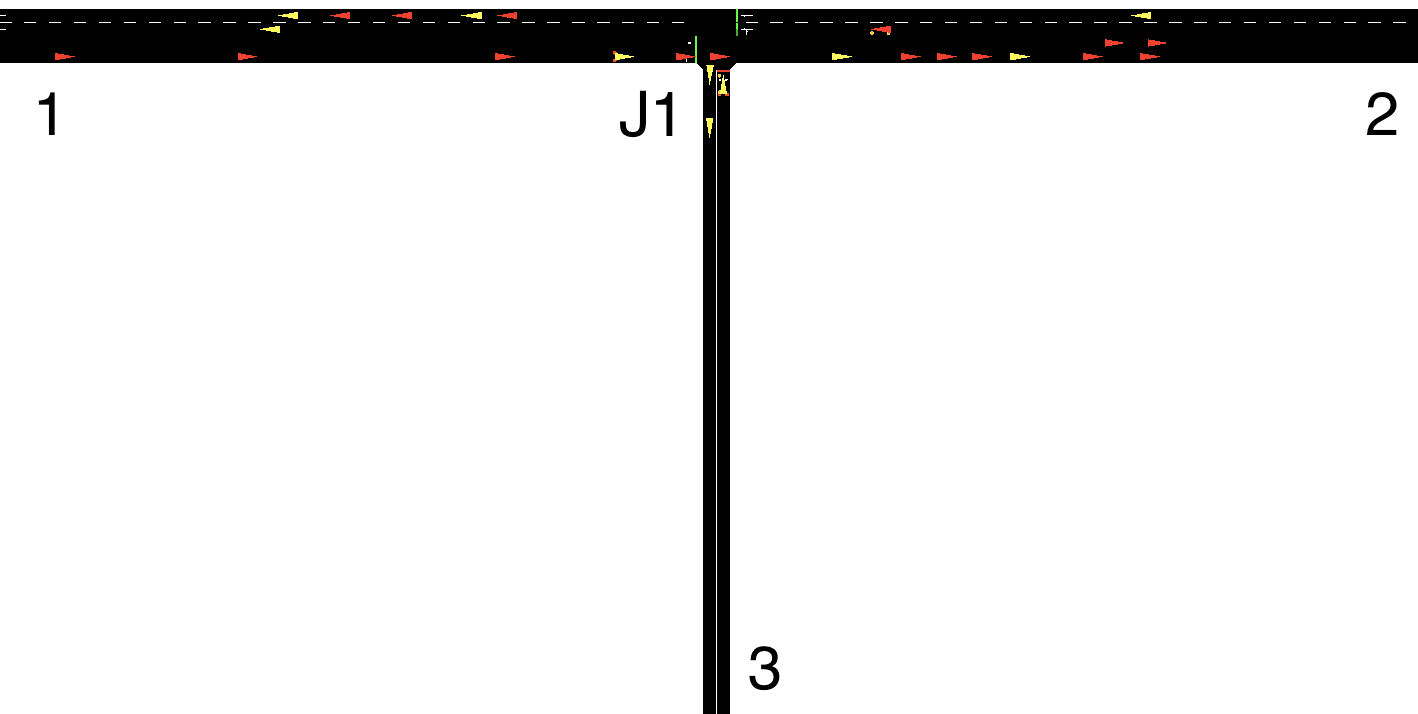
\includegraphics[width=0.2\paperwidth]{./pictures/simpleT2.png} &
		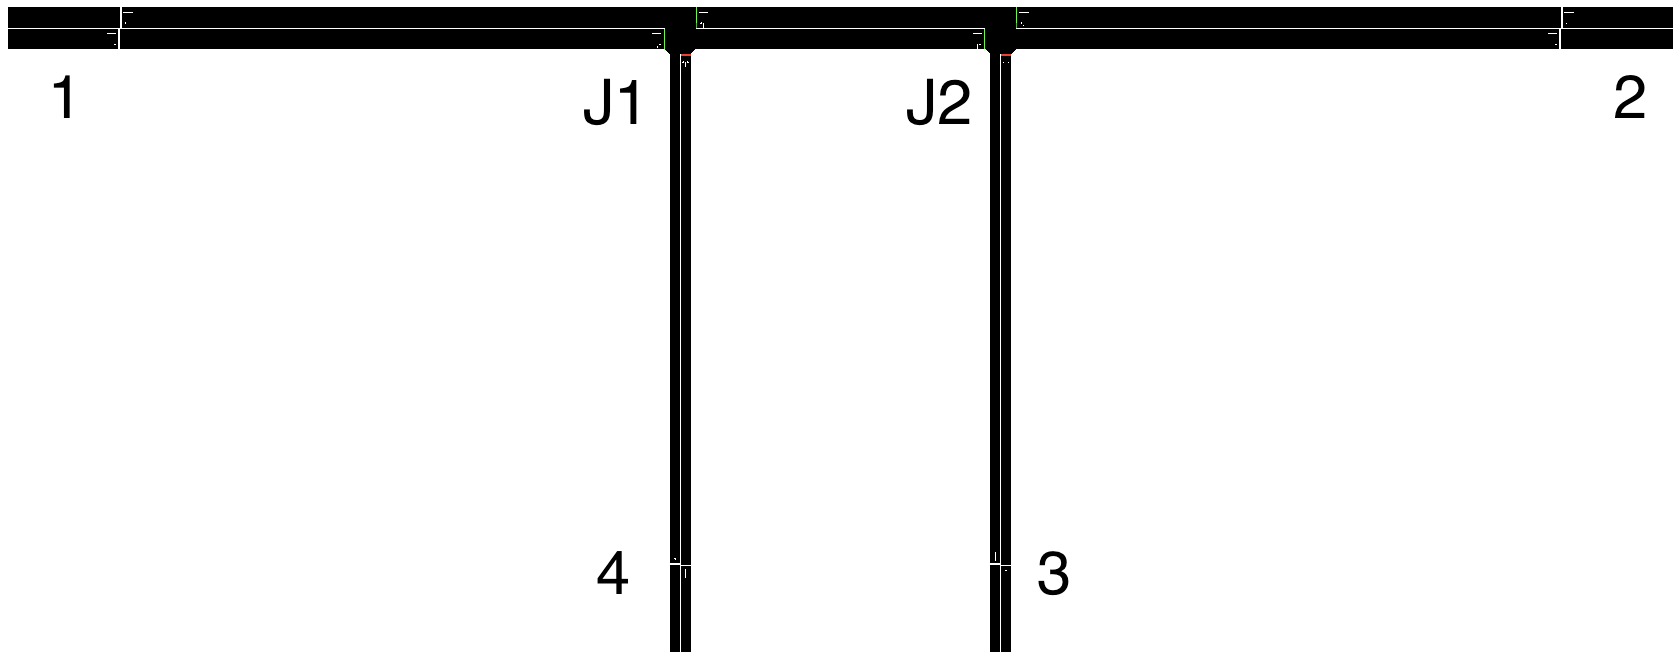
\includegraphics[width=0.26\paperwidth]{./pictures/twinT.png}\\
		\small\emph{(a)} & \small\emph{(b)} \\[0.1cm]
		\raisebox{0.9cm}{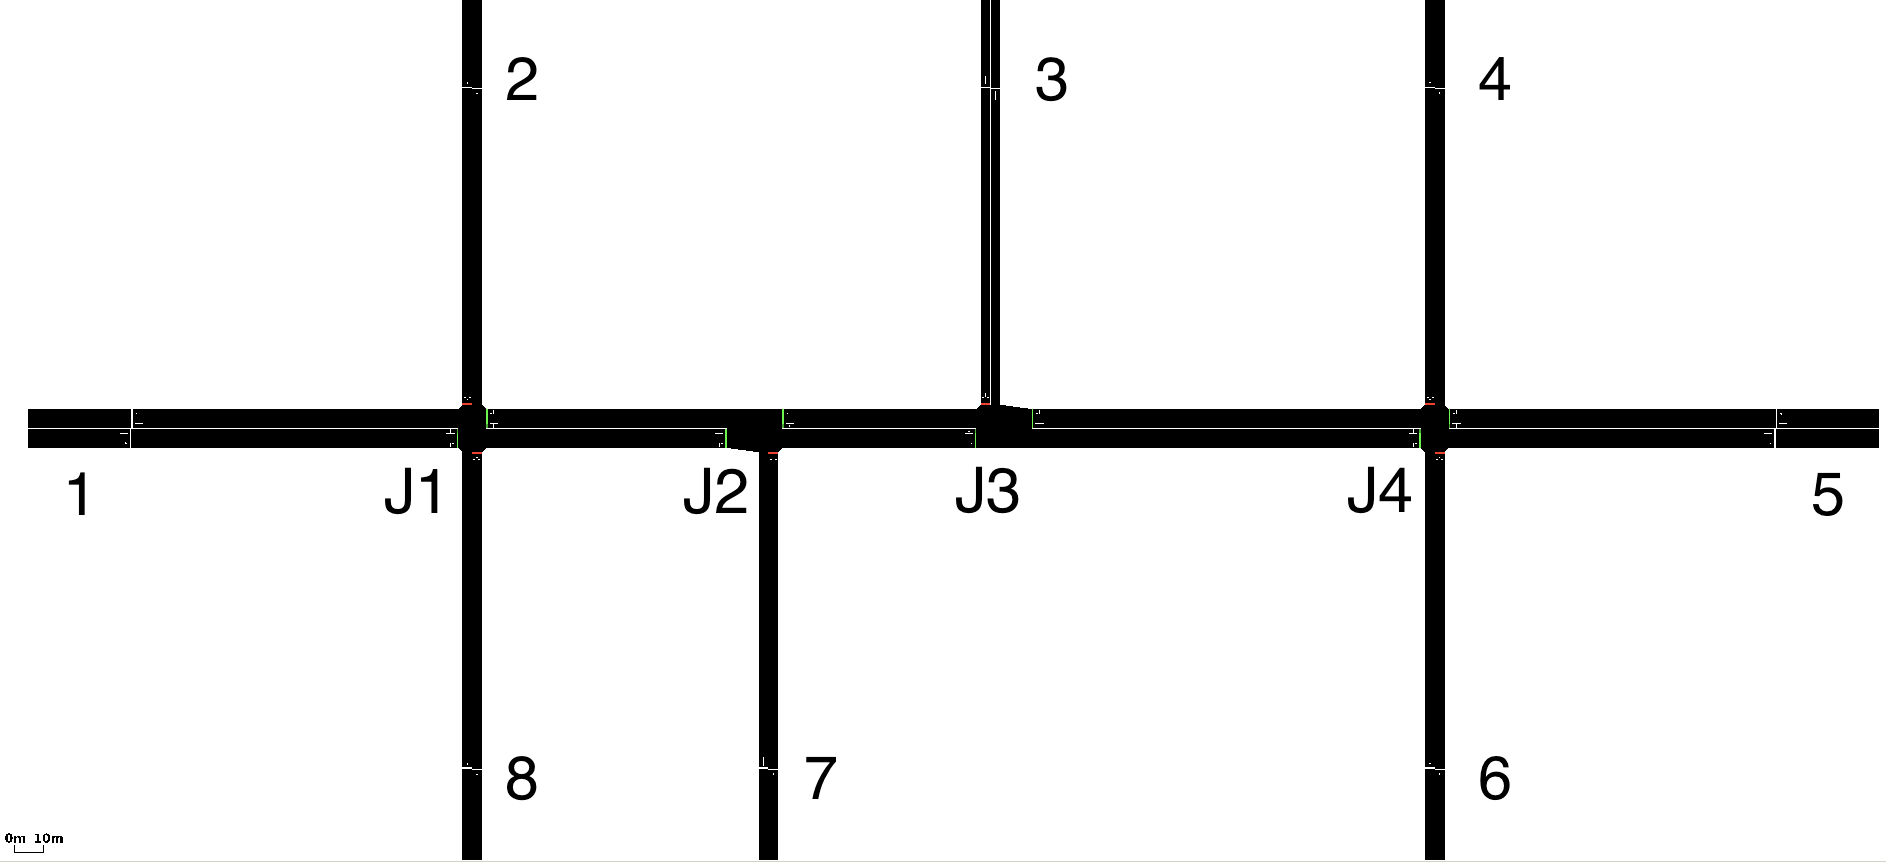
\includegraphics[width=0.25\paperwidth]{./pictures/corridor.png}}& 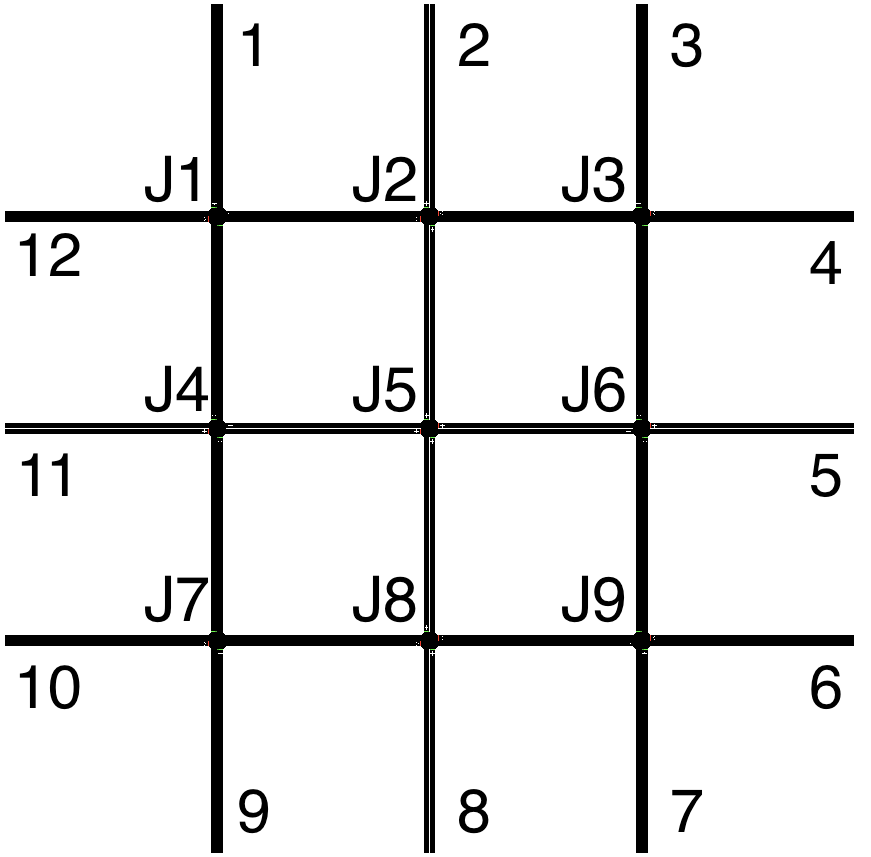
\includegraphics[width=0.2\paperwidth]{./pictures/manhattan.png} \\
		\small\emph{(c)} & \small\emph{(d)} \\[0.1cm]
	\end{tabular}
	\vspace{-5pt}
	\caption{The four road topologies used in the simulations. (a) Simple T-Junction, (b) Twin T-Junction, (c) Corridor, (d) Manhattan grid.}\label{fig:roads}
\end{figure}

\subsection{Car-following Parameters}
The Krauss~\cite{Krauss1998} microscopic car-following model was chosen as it produces stable collision-free traffic flow, and is well validated. As GPS-VA depends on information from CVs, the performance of the control strategies will depend on the penetration of CVs in the fleet. In order to model increasing CV penetration, two vehicle types are defined: Unconnected vehicles which do not support ITS functionality, and CVs capable of communicating CAMs. It is assumed that CVs do not have any driving advantages over unconnected vehicles. Therefore, both vehicle types have identical car-following parameters as described in Table~\ref{tab:vtype}. The only difference between the vehicle types is that CVs can broadcast ITS CAMs. The parameters in Table~\ref{tab:vtype} are typical of a passenger car.

\begin{table}[htb!]
	\small
	\centering
	\caption{The Krauss car-following model parameter values for both unconnected vehicles and CVs.\vspace{-1.ex}}
	\begin{tabular}{p{0.25\textwidth} >{\centering\arraybackslash}p{0.1\textwidth}}
		\toprule
		\textbf{Parameter} & \textbf{Value} \\\toprule
		Acceleration $(\m\sidiv\s^2)$ & 0.8 \\ \midrule
		Deceleration $(\m\sidiv\s^2)$ & 4.5 \\ \midrule
		Driver Imperfection - $\sigma$ & 0.5 \\ \midrule
		Reaction Time - $\tau(\s)$ & 1.0 \\ \midrule
		Length $(\m)$ & 5.0 \\ \midrule
		Min. Gap $(\m)$ & 2.5 \\ \midrule
		Max. Speed $(\m\sidiv\s)$ & 25 \\ 
		\bottomrule
	\end{tabular}
	\label{tab:vtype}
	%\vspace{-9pt}
\end{table}

\subsection{Traffic Generation}
Vehicle routes are randomly generated for each simulation run based on the probability of a vehicle travelling along a given route at rates of $\sim\!\!1500\ veh/h$ for approximately $3$ hours. The vehicles are randomly assigned a type (unconnected or CV) based on a CV penetration ratio from $0$ to $1$. The CV presence in the network is incremented from $0\%$ to $100\%$ in steps of $10\%$. As the proportion of CVs and the routes are defined at random, the experiments are repeated 15 times for each CV penetration to achieve reliable mean delays and confidence intervals. All random samples are uniformly distributed, and the random number generator for the route generation process is seeded using the run number so that the results are repeatable.

\subsection{Free-flow Travel Times}\label{sec:freeflow}
The free-flow travel time is the base on which the delay calculations in Section~\ref{sec:discussion} are made. Free-flow travel time is established by setting all intersection lights to green and passing $50$ cars along each route in all the models. The average free-flow travel time for each route is then established. The vehicle departures are spaced in time so that the vehicles do not interact. Additional time is added between the calculation of a subsequent route's free-flow time to allow vehicles from the previous test to clear the network.

\begin{figure*}[!tb]
	\begin{center} 
		\includegraphics[width=\textwidth]{./pictures/delay_grid.pdf}
		\vspace{-15pt}
		\caption{Travel-time delay for the intersection control strategies on each of the four road networks. The solid lines denote the mean delay over all the simulation runs. The dashed lines denote the 5th and 95th percentiles of the data as an indicator of travel time variability.}
		\label{fig:results}
	\end{center}
	\vspace{-5pt}
\end{figure*}

\section{Results and Discussion}\label{sec:discussion}
The proposed GPS-VA algorithm is tested against the fixed-time and Loop-VA control algorithms on four road network models at increasing levels of CV penetration. Where CV penetration is the percentage of vehicles in the network that are CVs. Figure~\ref{fig:results} shows a comparison of the delay times for each intersection control strategy on each road model. 

Travel-time delay characterises the excess time a vehicle takes to complete its journey compared to the free-flow travel time for the same journey. The simulation time $T_{\rm sim}$ is:
\begin{equation}
T_{\rm sim} = T_{\rm out} - T_{\rm add}
\end{equation}
where $T_{\rm add}$ is the time the vehicle is added to the simulation, and $T_{\rm out}$ is the time the vehicle exits the simulation. Time delay $T_{\rm Delay}$ can therefore be given by
\begin{equation}
T_{\rm Delay} = T_{\rm sim} - T_{\rm freeflow}
\end{equation}	
where $T_{\rm freeflow}$ is the time it takes the vehicle to make its journey on an unobstructed route. The free-flow travel times $T_{\rm freeflow}$ are as calculated in Section~\ref{sec:freeflow}. Delay time indicates the amount of time actually saved compared to the complete journey time, and highlights the performance limitations of each method.

Figure~\ref{fig:results} shows a comparison of the delay times for each intersection control strategy on each road model. It can be seen that in all cases, the traffic responsive actuated control strategies reduce delays better than the fixed-time algorithm. GPS-VA degenerates to fixed-time with minimum green time cycles and performs poorly at low CV penetrations. However, at CV penetration rates exceeding $30\%$, GPS-VA reduces delay comparably to or better than the implemented Loop-VA strategy for different traffic levels. GPS-VA's poor performance at low CV penetrations is expected, as the strategy degenerates to fixed time control with minimum green cycle phase lengths. The poor performance at low CV penetrations is a direct result of a control action deficit, and suggests that future work should investigate a system that uses both inductive loop and CAM information cooperatively to increase the algorithm's robustness. The Loop-VA and fixed-time strategies do not show as large a delay difference in the corridor model as in the other three. This is due to the short road segments connecting each junction inhibiting traffic flow. A coordinated strategy is more appropriate than isolated control in this case.

Discuss HVA1 and HVA2 results...

The reduction in delay with increasing CV penetration for GPS-VA is similar for road networks (a), (c), and (d), but much steeper for network (b). The alternative trend in the delay line on network (b) could be attributed to the proximity of the junctions, or more likely is due to the traffic demand levels applied to the network being too low to stress the junction adequately.

\section{Conclusions and Future Work}\label{sec:conclusion}
This paper explores how traffic responsive vehicle actuation for isolated intersection can be achieved using GPS and inductive loop data. The HVA algorithm uses position and heading data received from CV status broadcasts to actuate intersection signal timings by determining vehicle queue lengths and detecting vehicles passing through the intersection. Where CV data is unavailable the HVA algorithm attempts to use data from inductive loops to perform Loop-VA.

The HVA algorithm shows how data sources can be used together to achieve better control than either in isolation. HVA also demonstrates how multiple algorithms can be used and selected based on which provides the best solution for the current traffic demand. By using both GPS and loop data HVA provides the enhanced control afforded by ITS data streams, while remaining robust at low CV penetrations. In practice, the algorithm could be deployed in urban areas in the near future, and as the areas residents adopt CVs the control improves as people update their vehicles. This contrasts many of the current ITS based control algorithms which rely on high CV penetrations.

Microscopic simulations were performed to see how the proposed HVA algorithm using 1 and 2 inductive loops performs compared to fixed-time, Loop-VA,  and GPS-VA control strategies on four common urban road topologies. 
The results show that HVA is a compelling alternative to traditional intersection control strategies, showing delay reductions of $10\%-50\%$ over traditional Loop-VA for CV penetrations exceeding $30\%$.

Algorithms that incorporate data from CVs and that consider low CV fleet penetrations are still an underdeveloped research area. Further work needs to be done to investigate which ITS data streams are the most effective for signalised intersection control, and increase the robustness of control algorithms at low CV penetrations. Work also needs to be done to establish the effects of errors on the HVA algorithm. Communication packet loss, GPS measurement noise, and disparate GPS measurement rates all must be considered if the algorithm is to be robust in real road networks and reliably provide reduced travel times to drivers.

\section{Acknowledgements}
The authors would like to acknowledge support from the EPSRC and the Transport Research Laboratory (TRL) under Centre for Doctoral Training grant EP/L015382/1.

\newpage

\bibliographystyle{trb}
\bibliography{library}
\end{document}
